\documentclass[11pt,a4paper]{article}

% --- Packages ---
\usepackage[margin=1in]{geometry} % For page layout
\usepackage{graphicx}   % For including images
\usepackage{amsmath}    % For math symbols and equations
\usepackage{amssymb}
\usepackage{titlesec}
\usepackage{caption}    
\usepackage{subcaption} % <--- ADD THIS PACKAGE
\usepackage{listings}   % ADDED: Essential for R code

% --- Formatting ---
\titlespacing*{\section}{0pt}{1.2ex plus .2ex}{0.8ex plus .2ex}
\captionsetup{font=small,labelfont=bf,skip=4pt}

% --- Title Information ---
\title{Analysis of Annual Temperature Trend in Key West, Florida}
\author{Anaga Ambady}
\date{October 2025}

\begin{document}
\maketitle
\thispagestyle{empty} % No page number on the first page

% --- Section: Research Question ---
\section*{Is Florida Getting Warmer? A Permutation Test}

\subsection*{Methodology}
The null hypothesis ($H_0$) states that there is no correlation between year and annual mean temperature in Key West, Florida. 
Due to the lack of independence in a time series, a \textbf{permutation test} was used instead of the standard Pearson's p-value. 
The procedure involved calculating the observed correlation ($r_{\text{obs}}$) and comparing it to a distribution of 
$N = 10{,}000$ correlation coefficients generated by randomly re-assigning temperatures to years.

\subsection*{Results}
The observed correlation coefficient between Year and Temperature in Key West was:
\[
r_{\text{obs}} = 0.5331784
\]
The Monte Carlo p-value, calculated as the fraction of absolute permuted correlations 
($|r_{\text{perm}}|$) that were greater than or equal to $|r_{\text{obs}}|$, was:
\[
p < 0.0001
\]

\begin{figure}[t!] % [t!] prioritizes placing the figure at the absolute top of the page.
    \centering
    
    % --- ROW 1: Null Distribution Histogram (Largest Image) ---
    \begin{subfigure}{\textwidth} % Make the first plot occupy the full line
        \centering
        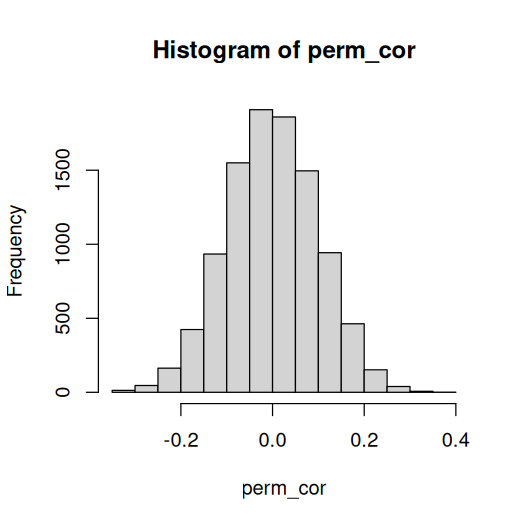
\includegraphics[width=0.65\textwidth]{../data/hist_cor.png} 
        \caption{Null Distribution of Correlation Coefficients from $N=10{,}000$ permutations. The observed correlation ($r_{\text{obs}} \approx 0.53$) is marked on the distribution.}
        \label{fig:histogram}
    \end{subfigure}
    
    \vspace{0.5\baselineskip} % Add a small vertical space between rows
    
    % --- ROW 2: Original and Permuted Scatter Plots (Small Images) ---
    \begin{subfigure}{0.45\textwidth} % Max width for scatter plot 1
        \centering
        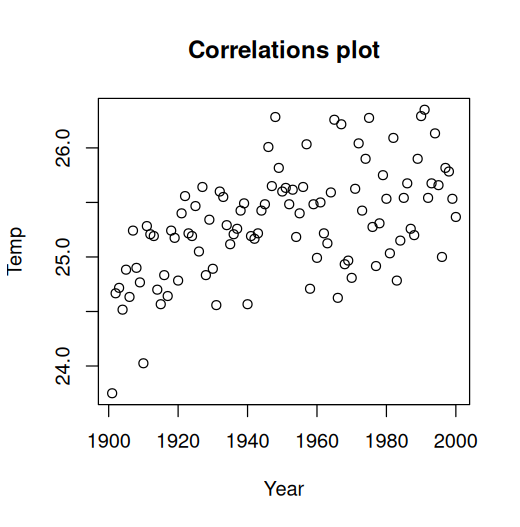
\includegraphics[width=0.85\linewidth]{../data/Rplot original plot.png} % Scale image relative to subfigure width
        \caption{Original Data Scatter Plot ($r_{\text{obs}} \approx 0.53$)}
        \label{fig:original_plot}
    \end{subfigure}%
    \hfill % Pushes the next subfigure to the right
    \begin{subfigure}{0.45\textwidth} % Max width for scatter plot 2
        \centering
        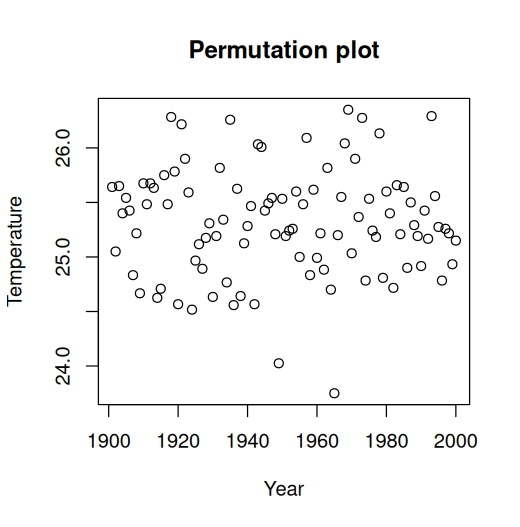
\includegraphics[width=0.85\linewidth]{../data/perm1.png}
        \caption{Example Permutation Scatter Plot ($r_{\text{perm}} \approx 0.05$)}
        \label{fig:perm_example}
    \end{subfigure}
    
    % Final main caption for all three parts
    \caption{Results of the Permutation Test. The distribution of $r_{\text{perm}}$ (A) demonstrates that the observed correlation ($r_{\text{obs}}$) is highly unlikely under the null hypothesis, as visualized by the original and permuted data plots (B and C).}
    \label{fig:all_plots}
\end{figure}
    
\subsection*{Interpretation}
The Monte Carlo p-value ($p < 0.0001$) indicates that less than 1 out of 10,000 random permutations resulted in a correlation coefficient as strong as the observed value ($r_{\text{obs}} \approx 0.53$). This provides **strong statistical evidence to reject the null hypothesis** ($H_0$) of no correlation. We conclude that there is a highly significant positive trend, suggesting that the annual mean temperature in Key West, Florida, is getting warmer.

\end{document}
